%%%%%%%%%%%%%%%%%%%%%%%%%%%%%%%%%%%%%%
% LaTeX poster template
% Created by Nathaniel Johnston
% August 2009
% http://www.nathanieljohnston.com/2009/08/latex-poster-template/
%%%%%%%%%%%%%%%%%%%%%%%%%%%%%%%%%%%%%%
\documentclass{beamer}
\usepackage[orientation=landscape,size=a0,scale=1.2]{beamerposter}
\usepackage{graphicx}			% allows us to import images
 
%-----------------------------------------------------------
% The packages used in our latex file
%-----------------------------------------------------------

\usepackage[T1]{fontenc}
\usepackage{amsmath,amssymb,amsthm}
\usepackage{mathtools}
\mathtoolsset{centercolon}
\usepackage{tikz}
\makeatletter
\protected\def\tikz@nonactivecolon{\ifmmode\mathrel{\mathop\ordinarycolon}\else:\fi} 
\makeatother
\usetikzlibrary{decorations.pathreplacing}
\usepackage{verbatim}
\usepackage[normalem]{ulem} 
\usepackage{thmtools}
\usepackage{color}
\usepackage[english]{babel}


%-----------------------------------------------------------
% Define the column width and poster size
% To set effective sepwid, onecolwid and twocolwid values, first choose how many columns you want and how much separation you want between columns
% The separation I chose is 0.024 and I want 4 columns
% Then set onecolwid to be (1-(4+1)*0.024)/4 = 0.22
% Set twocolwid to be 2*onecolwid + sepwid = 0.464
%-----------------------------------------------------------

\newlength{\sepwid}
\newlength{\onecolwid}
\newlength{\twocolwid}
\newlength{\threecolwid}
\setlength{\sepwid}{0.04\paperwidth}
\setlength{\onecolwid}{0.28\paperwidth}
\setlength{\twocolwid}{0.6\paperwidth}
\setlength{\threecolwid}{.92\paperwidth}
\setlength{\topmargin}{-0.5in}
\usetheme{confposter}
\usepackage{exscale}

%-----------------------------------------------------------
% The next part fixes a problem with figure numbering. Thanks Nishan!
% When including a figure in your poster, be sure that the commands are typed in the following order:
% \begin{figure}
% \includegraphics[...]{...}
% \caption{...}
% \end{figure}
% That is, put the \caption after the \includegraphics
%-----------------------------------------------------------

\usecaptiontemplate{
\small
\structure{\insertcaptionname~\insertcaptionnumber:}
\insertcaption}

%-----------------------------------------------------------
% Define colours (see beamerthemeconfposter.sty to change these colour definitions)
%-----------------------------------------------------------

\setbeamercolor{block title}{fg=ngreen,bg=white}
\setbeamercolor{block body}{fg=black,bg=white}
\setbeamercolor{block alerted title}{fg=white,bg=dblue!70}
\setbeamercolor{block alerted body}{fg=black,bg=dblue!10}

%%%%%%%%%%%%%%%%%%%%%%%%%%%%%%%%%%%%%%
% Miscellaneous Macros

\newcommand{\sbra}[1]{\langle{#1}|}
\newcommand{\sket}[1]{|{#1}\rangle}
\newcommand{\sbraket}[2]{\langle{#1}|{#2}\rangle}
\newcommand{\ceil}[1]{\lceil{#1}\rceil}
\newcommand{\CC}{\mathbb{C}}
\newcommand{\II}{\mathbb{I}}
\newcommand{\KK}{\mathbb{K}}
\newcommand{\QQ}{\mathbb{Q}}
\newcommand{\RR}{\mathbb{R}}
\newcommand{\ZZ}{\mathbb{Z}}
\newcommand{\posint}{\ZZ^+}
\renewcommand{\sc}{\mathrm{sc}}
\newcommand{\bc}{\mathrm{bc}}
\newcommand{\ph}{\mathrm{ph}}

\DeclareMathOperator{\spn}{span}


%-----------------------------------------------------------
% Name and authors of poster/paper/research
%-----------------------------------------------------------

\title{Momentum Switches}
\author{Andrew M. Childs$^{1,2}$, 
  David Gosset$^{1,2}$,\\ 
  Daniel Nagaj$^{3,4}$,
  Mouktik Raha$^{2,5}$, 
  and \underline{Zak Webb}$^{2,6}$} 

\institute{$^1$ Department of Combinatorics \& Optimization, University of Waterloo\\
  $^2$ Institute for Quantum Computing, University of Waterloo\\
  $^3$ Faculty of Physics, University of Vienna\\
  $^4$ Institute of Physics, Slovak Academy of Sciences\\
  $^5$ Department of Physics and Meteorology, Indian Institute of Technology Kharagpur\\
  $^6$ Department of Physics \& Astronomy, University of Waterloo}


\begin{document}

%----------------------------------------------------------
% Including the Logos
%----------------------------------------------------------

\addtobeamertemplate{headline}{} 
{
\begin{tikzpicture}[remember picture,overlay] 
\node [shift={(17.5 cm,-6.5cm)}] at (current page.north west) {
\includegraphics[height=15cm]{UW_Logo}}; 
\node [shift={(11.5 cm,-15cm)}] at (current page.north west) {
\includegraphics[height=8cm]{IQC_Logo}}; 

\node [shift={(-15.5 cm,-6.5cm)}] at (current page.north east) {
\includegraphics[height=6cm]{U_Vienna_Logo}}; 
\node [shift={(-17.5 cm,-15cm)}] at (current page.north east) {
\includegraphics[height=6cm]{IIT_Logo}}; 
\end{tikzpicture} 
}


\tikzset{global scale/.style={
    scale=#1,
    every node/.style={scale=#1}
  }
}
%-----------------------------------------------------------
% Start the poster itself
%-----------------------------------------------------------

\begin{frame}[t]
  \begin{columns}[t]												% the [t] option aligns the column's content at the top
    \begin{column}{\sepwid}\end{column}			% empty spacer column
    \begin{column}{\onecolwid}
      \begin{alertblock}{Abstract}
        Certain continuous-time quantum walks (CTQW) can be viewed as scattering processes. These processes can perform quantum computations, but it is challenging to design graphs with desired scattering behavior.
        \vspace{1cm}
        
        We study and construct momentum switches, graphs that route particles depending on their momenta. We also give an example where no exact momentum switch exists, although we construct arbitrarily good approximations.
      \end{alertblock}
    \end{column}
    
%%%%    

    \begin{column}{\sepwid}\end{column}
    \begin{column}{.72\twocolwid}
      \begin{block}{Graph Scattering}
      
        The Hamiltonian for CTQW is the adjacency matrix of the underlying graph.  For the infinite path, the (unnormalized) eigenvectors correspond to states with momenta $k\in [-\pi,\pi)$.
        \\~\\
        Given any finite graph $\hat{G}$, we can construct a scattering gadget by attaching several semi-infinite paths to $\hat{G}$.  Along the attached paths the eigenstates should be similar to the momentum states of the infinite path.  In fact, these eigenstates take the form of an incoming wave-packet traveling along one path, scattering off the graph, and traveling away from the graph in superposition over all the paths.  We will be interested in the cases where the transmission is perfect, such that all the scattering amplitude is contained on one path.
        \end{block}
      \end{column}
      
%%%%      
      
      \begin{column}{.05\twocolwid}\end{column}
      \begin{column}{.25\twocolwid}
      
      
      \begin{figure}
        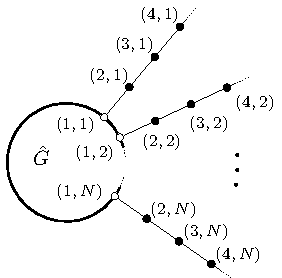
\includegraphics[width=.25\twocolwid]{scattering_graph.pdf}
      \end{figure}
      
      \end{column}
      
      \begin{column}{\sepwid}\end{column}
    \end{columns}
       
%%%%%----     
    
    
  \begin{columns}[t]
  \begin{column}{\sepwid}\end{column}
  \begin{column}{\onecolwid}
    \begin{block}{Momentum Switches}
        A momentum switch is a scattering gadget with three attached semi-infinite paths, such that at one momentum $k$ a particle transmits perfectly from path 1 to path 2, while at another momentum $p$ the particle transmits perfectly from path 1 to path 3.  These can be used to construct momentum dependent unitaries.
       
       \begin{figure}
         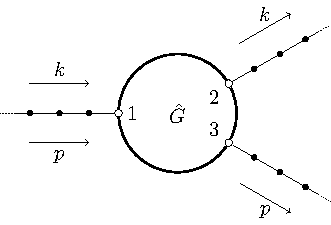
\includegraphics[height=.25\onecolwid]{momentum_switch.pdf}
       \end{figure}
        
        
    \end{block}
  \end{column}
    \begin{column}{\sepwid}\end{column}
    \begin{column}{\twocolwid}
      \begin{block}{Our Construction}
        To construct momentum switches between two momenta, it suffices to find a particular two-terminal gadget (called a type 2 R/T gadget). Such a gadget consists of some finite graph $\tilde{G}$ attached to an infinite path by one edge.  The scattering behavior for such a gadget depends on the form of the eigenstates of $\tilde{G}$, allowing for explicit modifications.  Given such a graph that reflects at one momentum and transmits at another, we can explicitly construct another gadget that interchanges the two momenta, and a momentum switch between them.
      \end{block}
      \begin{columns}[t]
      \begin{column}{.5\onecolwid}
        \begin{figure}
          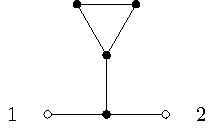
\includegraphics[height=.25\onecolwid]{example_rt.pdf}
          \caption{An R/T gadget that transmits at $-\frac{\pi}{3}$ and reflect at $-\frac{2\pi}{3}$.}
        \end{figure}
      \end{column}
      \begin{column}{\sepwid}
      \end{column}
      \begin{column}{.5\onecolwid}
        \begin{figure}
          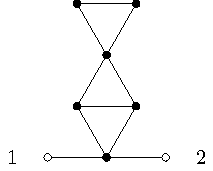
\includegraphics[height=.25\onecolwid]{example_tr.pdf}
          \caption{A related gadget that reflects at $-\frac{\pi}{3}$ and transmits at $-\frac{2\pi}{3}$.}
        \end{figure}
      \end{column}
      \begin{column}{\sepwid}
      \end{column}
      \begin{column}{.5\onecolwid}
        \begin{figure}
          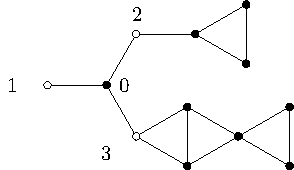
\includegraphics[height=.25\onecolwid]{example_switch.pdf}
          \caption{A momentum switch between $-\frac{\pi}{3}$ and $-\frac{2\pi}{3}$.}
        \end{figure}
      \end{column}
      \end{columns}
    \end{column}
    \begin{column}{\sepwid}\end{column}
  \end{columns}
  
  \begin{columns}[t]
    \begin{column}{\sepwid}\end{column}
    \begin{column}{\onecolwid}
      \begin{block}{Impossibility Results}
          The existence of a momentum switch implies the existence of an R/T gadget, by simply removing one of the attached paths.  Hence, by showing that no R/T gadget exists between momenta $-\frac{\pi}{4}$ and $-\frac{3\pi}{4}$, we show that no momentum switch exists either.  
          \\~\\          
          To show that no R/T gadget exists, we first show that there exists a basis for the scattering states where amplitudes are from $\QQ[\sqrt{2}]$.  We then use this basis to show that if a gadget perfectly reflects at momentum $-\frac{\pi}{4}$, then it also perfectly reflects at momentum $-\frac{3\pi}{4}$.
          
       \end{block}
    \end{column}
    
    \begin{column}{\sepwid}\end{column}
    \begin{column}{\onecolwid}
     \begin{block}{Approximate Switch}
        While we showed that no exact momentum switch can exist between $-\frac{\pi}{4}$ and $-\frac{3\pi}{4}$, we do construct an approximate switch with arbitrary precision. 
        \\~\\
        This proceeds by an interferometry process, in which the incoming particle is split onto two paths, and a momentum dependent phase is applied along one of the paths.  When the two paths are then recombined, the output is concentrated on path 2 or 3 depending on the incoming momentum.  
      \end{block}
    \end{column}
    
    \begin{column}{\sepwid}\end{column}
    \begin{column}{\onecolwid}
      \begin{block}{Acknowledgements}
         \footnotesize{This work was supported in part by NSERC; the Ontario Ministry of Research and Innovation; the Ontario Ministry of Training, Colleges, and Universities; the US ARO; and the Slovak Research and Development Agency brant APVV-0808-12 QIMABOS.}
      \end{block}
      
      \begin{block}{References}
        \bibliographystyle{myhamsplain}
        \nocite{*}
        \footnotesize{\bibliography{mom_switch.bib}}
      \end{block}
      
    \end{column}  
    
    \begin{column}{\sepwid}\end{column}
  \end{columns}     

      
    
\end{frame}
\end{document}